\section{MIP on arbitrary polygonal cells}
In this section, we introduce the PieceWise Linear Discontinuous (PWLD) finite
elements developed in \cite{pwld_2d,pwld_3d,pwld_diffusion}. To define PWLD
basis functions for two-dimensional polygons, we first divide each polygonal
cell into ``side'' sub-cells. A ``side'' sub-cell is a triangle made from two
adjacent vertices and the within-cell point $c$. The coordinates of $c$ are weighted
averages of the vertex coordinates:
\begin{align}
& x_c = \sum_{j=1}^{V} \alpha_{j} x_j\\
& y_c = \sum_{j=1}^{V} \alpha_{j} y_j
\end{align}
where $\sum_{j=1}^{V} \alpha_{j}=1$ and $V=$ number of vertices of the cell.\\
The basis function at vertex $j$ is defined as \cite{pwld_2d}:
\begin{equation}
b_{j} (x,y) = t_{j}(x,y) + \alpha_j t_c(x,y)
\end{equation}
where the $t_j$ functions are standard linear functions on triangles: $t_j
(x,y)$ is unity at vertex $j$; zero at $j-1$, $j+1$ and $c$; and zero in all
triangular sides that are not in contact with vertex $j$. The function $t_c
(x,y)$ is unity at $c$ and zero at each vertex. The parameters $\alpha_{j}$
are arbitrary positive weights. In this paper, we have always used 
$\alpha_{j}=\frac{1}{V}$. On a square cell with $\alpha_{j}=0.25\ \forall j$, 
the basis functions are given in Figure (\ref{pwld}):
\begin{figure}[H]
\centering
\subfloat[First basis function]{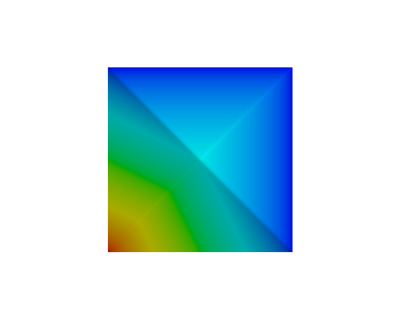
\includegraphics[width=0.3\textwidth]{pwld_1}}
\subfloat[Second basis function]{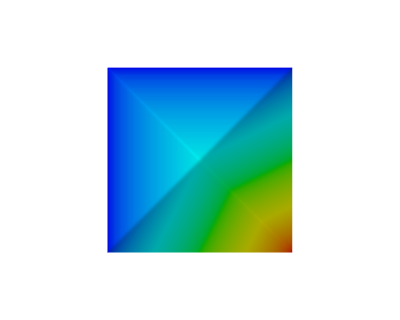
\includegraphics[width=0.3\textwidth]{pwld_2}}\\
\subfloat[Third basis function]{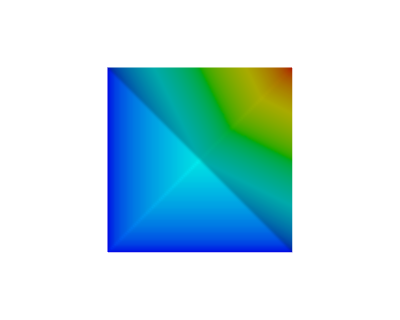
\includegraphics[width=0.3\textwidth]{pwld_3}}
\subfloat[Fourth basis function]{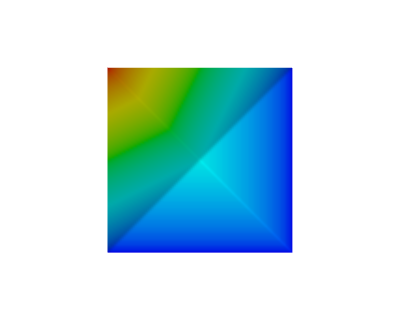
\includegraphics[width=0.3\textwidth]{pwld_4}}
\caption{PWLD basis function}
\label{pwld}
\end{figure}
It is interesting to note that on triangular cells, the PWLD basis functions
reduces to the standard LD basis functions. Since the PWLD basis functions are
built on triangular ``side'' sub-cells, the integrals over the area of a cell
is replaced by a sum of integrals over the sides of the cell. The PWLD method has 
a second-order convergence rate.

Having defined the spatial discretization that we will used, we can now
define the Modified Interior Penalty DSA \cite{mip}. This DSA scheme uses 
discontinuous Galerkin finite elements for the spatial discretization and has
been shown to be always stable for isotropic scattering on triangular cells. 
The MIP weak form can be written as:
\begin{equation}
b(\phi,\phi^*) = l(\phi^*)
\end{equation}
with:
\begin{equation}
\begin{split}
b(\phi,\phi^*) =& \(\Sigma_a \phi,\phi^*\)_{\mc{D}}+
(\mathrm{D}\bn\phi,\bn\phi^*)_{\mc{D}} + \(\kappa_e \llb\phi\rrb,
\llb\phi^*\rrb\)_{E_h^i} + \(\llb\phi\rrb,\ldb\mathrm{D}\partial_n\phi\rdb\)_{E_h^i} 
+\\
& \(\ldb\mathrm{D}\partial_n \phi\rdb,\llb\phi^*\rrb\)_{E_h^i} + \(\kappa_e
\phi,\phi^*\)_{\partial \mc{D}^d} -\frac{1}{2} \(\phi,\mathrm{D} \partial_n
\phi^*\)_{\partial \mc{D}^d} - \frac{1}{2}\(\mathrm{D}\partial_n
\phi,\phi^*\)_{\partial \mc{D}^d}
\label{mip_b}
\end{split}
\end{equation}
\begin{equation}
l(\phi^*) = (Q_0,\phi^*)_{\mc{D}}+ (J^{inc},\phi^*)_{\partial \mc{D}^r}
\label{mip_l}
\end{equation}
where $(f,g)_{\mc{D}} = \sum_{K\in \mathbb{T}_h} \(f,g\)_K$, 
$(f,g)_K = \int_K fg\ d\br$, $(f,g)_{E_h^i}=\sum_{e\in E_h^i}(f,g)_e$, 
$(f,g)_e = \int_e fg\ ds$, $Q_0 = \Sigma_{s,0} \delta \phi^{(l)}$, 
$J^{inc} = \sum_{\bo\cdot\bs{n}_b >0} w_m |\bo_m \cdot \bs{n}_b| \delta
\psi_m^{(l)}$, $\mathbb{T}_h$ is the mesh used to discretize the domain
$\mc{D}$ into nonoverlapping elements $K$, $E_h^i$ is the set of interior
edges, $\mc{D}$  is the spatial domain, $\partial \mc{D}^d$ is the boundary of
the domain with Dirichlet condition, $\partial \mc{D}^r$ is the boundary of
the domain with reflective condition, $\Sigma_a$ is the absorption macroscopic
cross section, D is the boundary coefficient, $\partial_n = \bs{n}\cdot \bn$
where $\bs{n}$ is the outward unit normal, $\llb\phi\rrb = \phi^+ - \phi^-$ is
the jump of $\phi$ at the interface between two elements, $\ldb\phi\rdb =
\frac{\phi^+ + \phi^-}{2}$ is the mean of $\phi$ at the interface between two
elements, $\phi^{\pm}=\lim_{s\rightarrow^{\pm}}\phi(\bs{r}+s\bs{n}_e)$,
$\bs{n}_e$ is the normal unit vector associated with a given edge $e$ and:
\begin{equation}
\kappa_e = \max\(\kappa_e^{IP},\frac{1}{4}\)
\end{equation}
with $\kappa_e^{IP} = \left\{
\begin{aligned}
&\frac{c(p^+)}{2} \frac{\mathrm{D^+}}{h_{\bot}^+} + \frac{c(p^-)}{2}
\frac{\mathrm{D}^-}{h_{\bot}^-} & \textrm{on interior edges, i.e., }
e\in E_h^i\\
&c(p) \frac{\mathrm{D}}{h_{\bot}} & \textrm{on boundary edges, i.e., } e
\in\partial \mc{D}^d 
\end{aligned}
\right. $
where $c(p)$ is given by $c(p) = 2p (p+1)$, $p$ is the polynomial order ($p=1$
in this paper) and $h_{\bot}$ is the length of the cell in the direction
orthogonal to the edge $e$. On triangle, $h_{\bot}=\frac{2a}{L_e}$ with $a$
the area of the triangle and $L_e$ the length of the edge $e$.

Using PWLD finite elements, \cref{mip_b,mip_l} become:
\begin{equation}
\begin{split}
b(\phi,\phi^*) =& \la\Sigma_a \phi,\phi^*\ra_{\mc{D}}+
\la\mathrm{D}\bn\phi,\bn\phi^*\ra_{\mc{D}} + \(\kappa_e \llb\phi\rrb,
\llb\phi^*\rrb\)_{E_h^i} + \la\llb\phi\rrb,\ldb\mathrm{D} 
\partial_n\phi\rdb\ra_{E_h^i} +\\
& \la\ldb\mathrm{D}\partial_n \phi\rdb,\llb\phi^*\rrb\ra_{E_h^i} + \(\kappa_e
\phi,\phi^*\)_{\partial \mc{D}^d} -\frac{1}{2} \la\phi,\mathrm{D} \partial_n
\phi^*\ra_{\partial \mc{D}^d} - \frac{1}{2}\la\mathrm{D}\partial_n
\phi,\phi^*\ra_{\partial \mc{D}^d}
\label{mip_b_pwld}
\end{split}
\end{equation}
\begin{equation}
l(\phi^*) = \la Q_0,\phi^*\ra_{\mc{D}}+ \(J^{inc},\phi^*\)_{\partial \mc{D}^r}
\label{mip_l_pwld}
\end{equation}
where $\la f,g\ra_{\mc{D}} = \sum_{K\in \mathbb{T}_h} \la f,g\ra_{K}$, 
$\la f,g \ra_K = \sum_{s=1}^{V_K} \int_{K_s} fg\ d\br$, $\la f, \partial_n g
\ra_{E_h^i} = \sum_{e\in E_h^i} \int_e \sum_{s}^{V_{K_g}} f\partial_n g\ ds$, 
$K_s$ is a ``side'' sub-cell, $V_K$ is the number of vertices of cell $K$ and
$K_g$ is the cell associate to edge where $g$ is defined.
When the cell are not triangular, there is no simple way to calculate
$h_{\bot}$. To simplify the calculation of $h_{\bot}$, we will assume that the
polygonal cells are not too far from being regular polygonal cells. Therefore,
$h_{\bot}$ is given by:
\begin{description}
\item[Triangular cell:] $h_{\bot} = 2\times \frac{area}{L_i}$
\item[Quadrilateral cell:] $h_{\bot} = \frac{area}{L_i}$
\item[Cell with even number of edges:] the orthogonal length is two times the 
apothem (inradius): $\textrm{apothem} = 2 \times
\frac{\textrm{area}}{\textrm{perimeter}} \Longrightarrow h_{\bot}= 4 \times
\frac{\textrm{area}}{\textrm{perimeter}}$
\item[Odd number of edges:] the orthogonal length is the apothem + the circumradius 
($r$): $r = \sqrt{\frac{2\times\textrm{area}}{N\sin\(\frac{2\pi}{N}\)}}
\Longrightarrow h_{\bot} = 2 \times \frac{area}{perimeter}+\sqrt{\frac{2\times
\textrm{area}}{N\sin\(\frac{2\pi}{N}\)}}$
\end{description}

